\documentclass[12pt]{article}

% Load packages
\usepackage{cite}              % Make references as [1-4], not [1,2,3,4]
\usepackage{url}              	% Formatting web addresses
\usepackage{ifthen}           	% Conditional
\usepackage{multicol}			% Multi-column pages
\usepackage[utf8]{inputenc}   	% Unicode support
\usepackage{amsmath}           % Support for writing math formulas
\usepackage{amssymb}           % Support for writing math formulas
\usepackage{epsfig}            % Support separate PostScript files for figs
\usepackage{epstopdf}			% Converts eps figs to pdf
\usepackage{graphicx}			% Graphics functions
\usepackage[margin=0.1pt,font=footnotesize,labelfont=bf]{caption}
% \usepackage{caption}			% Styles figure captions
\usepackage{setspace}			% Provides line spacing environments
\usepackage{colortbl}
\usepackage[wide]{sidecap}		% Can typeset caption aside the figure, allows use of margin for figs wider than \textwidth.
\usepackage[square,sort,comma,numbers]{natbib}
% \usepackage[authoryear,square,comma,sort&compress]{natbib}
\usepackage{supertabular}		% Tables spanning multiple pages
\usepackage{comment}
\usepackage{lineno}
\urlstyle{rm}					% URL style
\usepackage{wrapfig}			% Wrap text around figures
\usepackage[FIGTOPCAP,nooneline]{subfigure}
\captionsetup{font={scriptsize},aboveskip=0pt}	% Styles figure captions
\usepackage{simplemargins}
\setallmargins{1.0in}         % Set all margins
% \setlength\bibsep{0pt}     % Single spaced bib
\date{}
\doublespacing
% \singlespacing
\frenchspacing     % Eliminates double spaces between sentences

\makeatletter
\renewcommand\subsection{\@startsection
	{subsection}{2}{0mm}
	{-0.05in}
	{-0.5\baselineskip}
	{\normalfont\normalsize\bfseries}}
\renewcommand\subsubsection{\@startsection
	{subsubsection}{2}{0mm}
	{-0.05in}
	{-0.5\baselineskip}
	{\normalfont\normalsize\itshape}}
\renewcommand\section{\@startsection
	{subsection}{2}{0mm}
	{-0.2in}
	{0.05\baselineskip}
	{\normalfont\large\bfseries}}	
\renewcommand\paragraph{\@startsection
	{paragraph}{2}{0mm}
	{-0.05in}
	{-0.5\baselineskip}
	{\normalfont\normalsize\itshape}}
\makeatother

\newboolean{publ}

%Publication style settings
%\newenvironment{bmcformat}{\fussy\setboolean{publ}{true}}{\fussy}
\renewcommand{\rmdefault}{phv}\renewcommand{\sfdefault}{phv}
\renewcommand{\bibnumfmt}[1]{#1.}    % Change the number format in the ref list
\renewcommand{\figurename}{Fig.}     % Change Figure to Fig.

%%%%%%%%%%%%%%%%%%%%%%%%%%%%%%%%%%%%%%%%%%%%%%%%%%%%%%%%%%%%%%%%%%%%%
%%%%%%%%%%%%%%%%%%%%%%%%%%%%%%%%%%%%%%%%%%%%%%%%%%%%%%%%%%%%%%%%%%%%%

\begin{document}

%%%%%%%%%%%%%%%%%%%%%%%%%%%%%%%%%%%%%%%%%%%%%%%%%%%%%%%%%%%%%%%%%%%%%
% SUPPLEMENTARY MATERIAL
%%%%%%%%%%%%%%%%%%%%%%%%%%%%%%%%%%%%%%%%%%%%%%%%%%%%%%%%%%%%%%%%%%%%%
\section*{Supplementary Materials}

\begin{figure}[b]\centering
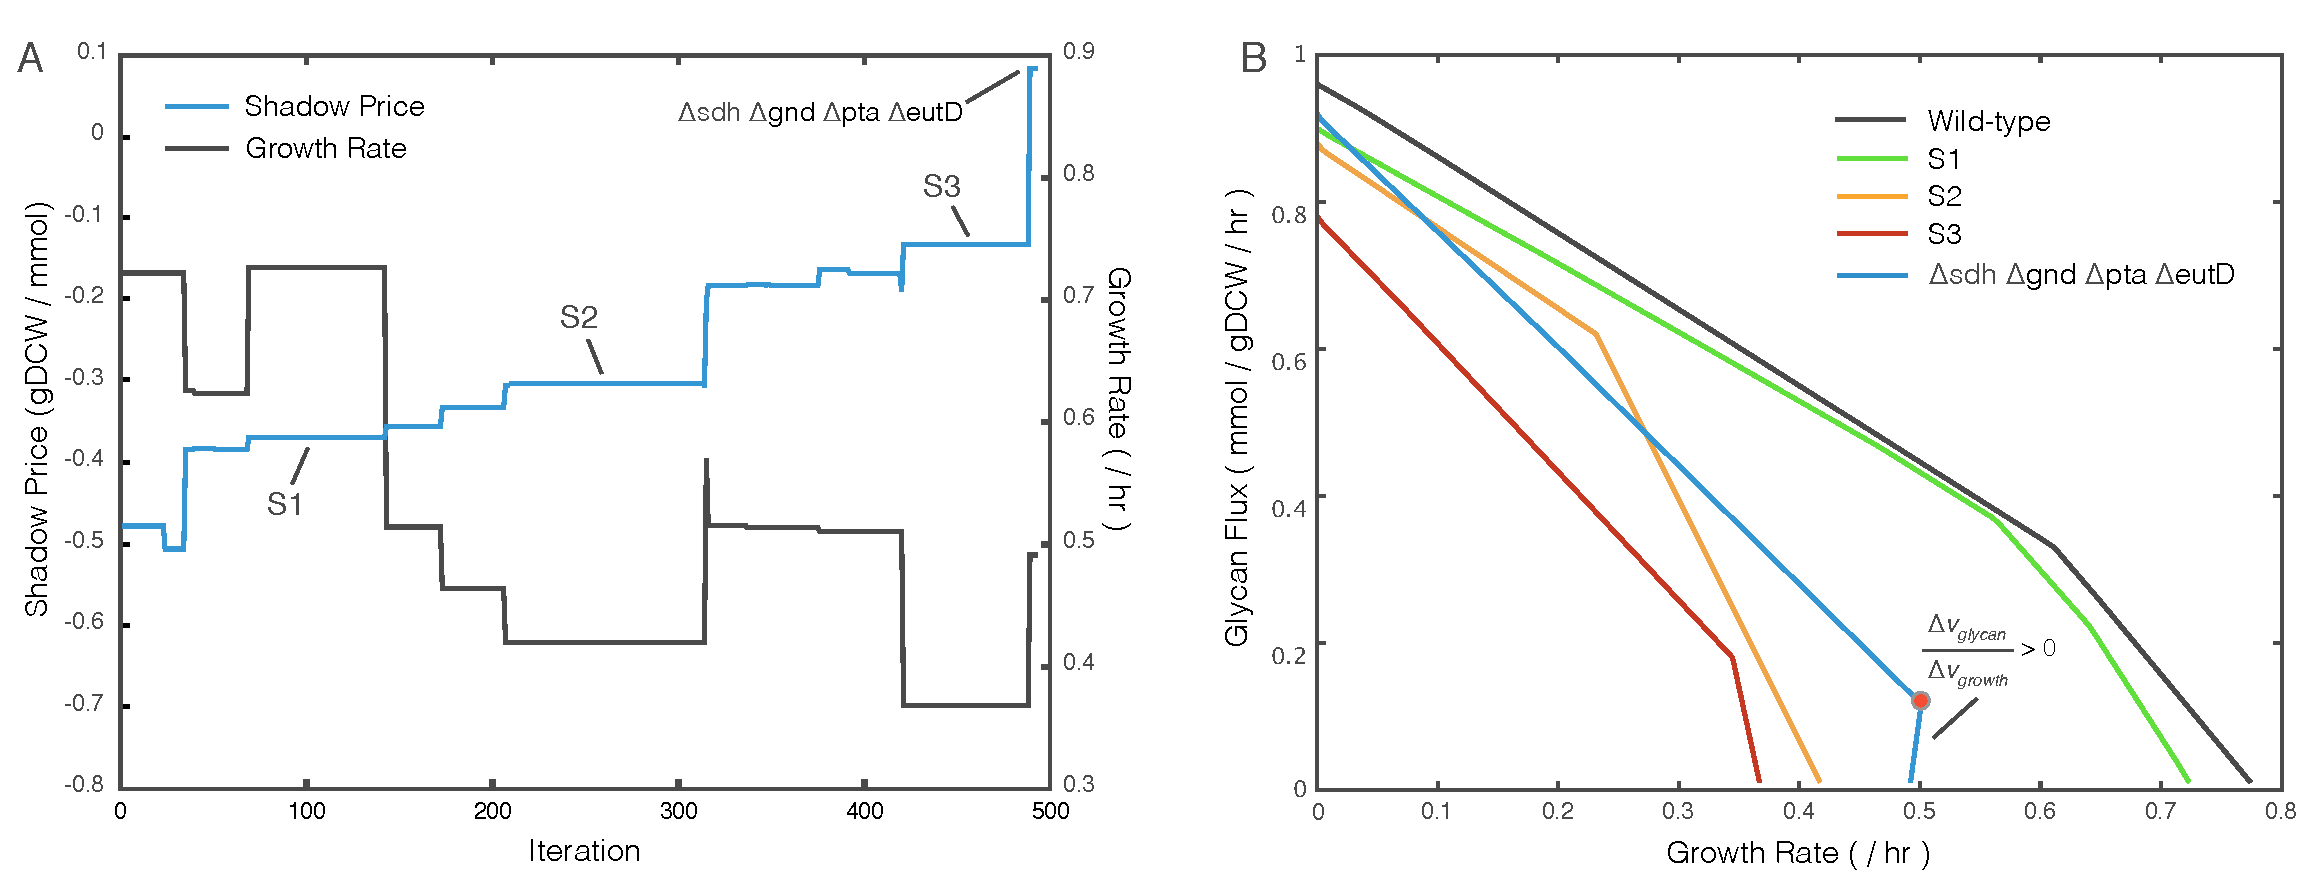
\includegraphics[width=1.0\textwidth]{./figures/sup-fig1-prod-env-single.pdf}
\caption{Representative simulated annealing simulation results identifying a growth-coupled strain of type EcM1. \textbf{(A)} Shadow price and FBA-maximized growth rate versus iteration identifying strain $\Delta$\textit{sdh}$\Delta$\textit{gnd}$\Delta$\textit{pta}$\Delta$\textit{eutD}. \textbf{(B)} Production envelopes of the strains at iteration points indicated in A. The simulation is terminated once a positive shadow price is found, visualized by the slope of the production envelope. The red dot indicates the optimal operating point of maximal growth rate for the growth-coupled strain.}
\label{fig:CH2-prod-env-single}
\end{figure}

%%%%%%%%%%%%%%%%%%%%%%%%%%%%%%%%%%%%%%%%%%%%%%%%%%%%%%%%%%%%%%%%%%%%%

\newpage
%\bibliographystyle{nature}
%\bibliography{Paper_2015_Ec_glyco_ref}

\end{document}
